\section{Como se hizo}

Para realizar el código se utilizo lo visto en la clase de \textit{introducción a la programación}, la mayor parte del funcionamiento del código se basa en \textit{bucles} y \textit{if}:

\begin{figure}[h]
    \raggedright
    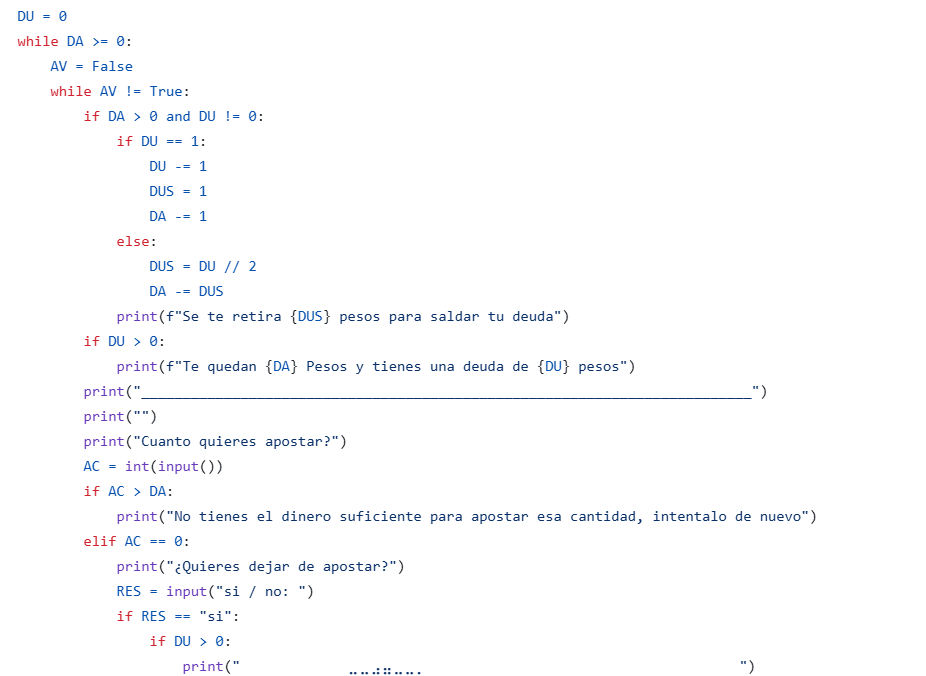
\includegraphics[width=0.5\linewidth]{Imagenes/C1.PNG}
\end{figure}

También se uso \textit{ASCII art} para darle mas personalidad al juego y retener la atención del jugador:

\begin{figure}[h]
    \raggedright
    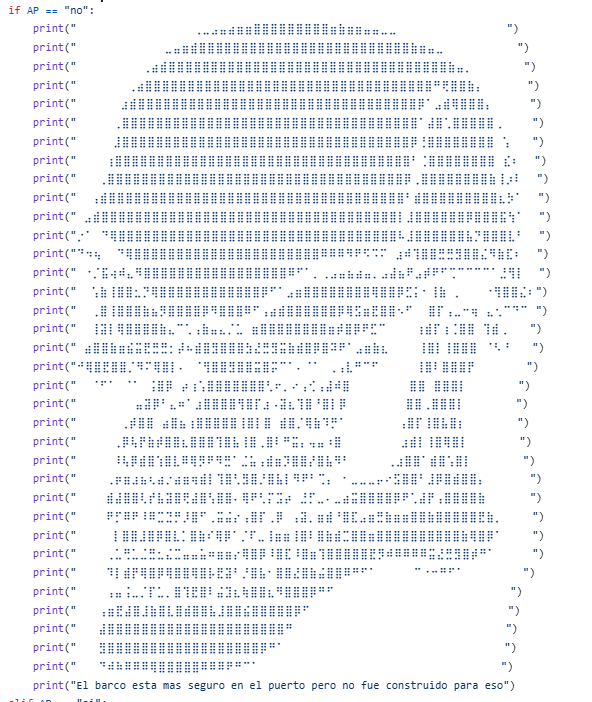
\includegraphics[width=0.5\linewidth]{Imagenes/C2.PNG}
\end{figure}

Todo el código se basa en lo anterior conectado uno tras otro hasta que tome forma.